\title{Basic Lessons on High School Olympiad 3}
\date{\today}
\author{Azzam L. H.}
\maketitle
\renewcommand*\contentsname{Daftar Isi}
\tableofcontents

\newpage
\section{Aljabar}
\subsection{Ketaksamaan}
\subsubsection{QM-AM-GM-HM}
Untuk bilangan real positif $a_1,a_2,\dots,a_n$ dengan $n\ge 2$,definisikan
\begin{align*}
    QM \text{ (Quadratic Mean) } &= \sqrt{\dfrac{a_1^2+a_2^2+\dots+a_n^2}{n}}\\
    AM \text{ (Arithmetic Mean) } &= \dfrac{a_1+a_2+\dots+a_n}{n}\\
    GM \text{ (Geometric Mean) } &=
    \sqrt[n]{a_1a_2\dots a_n}\\
    HM \text{ (Harmonic Mean) } &=
    \dfrac{n}{\dfrac{1}{a_1}+\dfrac{1}{a_2}+\dots+\dfrac{1}{a_n}}
\end{align*}

Maka berlaku $QM \ge AM \ge GM \ge HM$ atau 
$$\sqrt{\dfrac{a_1^2+a_2^2+\dots+a_n^2}{n}} \ge  \dfrac{a_1+a_2+\dots+a_n}{n}\ge
    \sqrt[n]{a_1a_2\dots a_n} \ge
    \dfrac{n}{\dfrac{1}{a_1}+\dfrac{1}{a_2}+\dots+\dfrac{1}{a_n}}$$
dengan kesamaan terjadi jika dan hanya jika $a_1=a_2=\dots =a_n$.
\subsubsection{Cauchy-Schwarz}
Untuk bilangan real $a_1,a_2,\dots,a_n$ dan $b_1,b_2,\dots,b_n$ berlaku
$$(a_1^2+a_2^2+\dots+a_n^2)(b_1^2+b_2^2+\dots+b_n^2) \ge (a_1b_1+a_2b_2+\dots+a_nb_n)^2$$

dengan kesamaan terjadi jika dan hanya jika $\dfrac{a_1}{b_1}=\dfrac{a_2}{b_2}=\dots =\dfrac{a_n}{b_n}$.

\subsubsection{Ketaksamaan Bernoulli}
Untuk $x > -1$ berlaku $(1+x)^n \ge 1+nx$.

\subsection{Ketaksamaan Kuadrat}
Untuk $x \in \RR$, berlaku kuadrat sempurnanya selalu nonnegatif atau $x^2 \ge 0$. Hal ini menyebabkan fungsi kuadrat $f(x)=ax^2+bx+c$ untuk $a \neq 0$ selalu mempunyai nilai minimum atau maksimum saat $x = -\dfrac{b}{2a}$. (why?)


\subsection{Floor and Ceiling}
Definisikan $\floor{x}$ (\textit{floor} $x$) sebagai bilangan bulat terbesar yang kurang dari sama dengan $x$. Simpelnya, $\floor{x}$ dapat dikatakan sebagai "pembulatan ke bawah". Contoh: $\floor{\pi}=3$, $\floor{2}=2$, $\floor{10,51}=10$, $\floor{-1,5}=-2$.

Definisikan $\ceiling{x}$ (\textit{ceiling} $x$) sebagai bilangan bulat terkecil yang lebih dari sama dengan $x$. Simpelnya, $\ceiling{x}$ dapat dikatakan sebagai "pembulatan ke atas". Contoh: $\ceiling{\pi}=4$, $\ceiling{2}=2$, $\ceiling{10,51}=11$, $\ceiling{-1,5}=-1$.

Definisikan $\{x\}$ sebagai \textit{fractional part} dari $x \in \RR$ dimana $\{x\} = x - \floor{x}$.

Beberapa properti:
\begin{enumerate}
    \item $\floor{x}=\ceiling{x}$ untuk $x \in \ZZ$.
    \item $\floor{x}=\ceiling{x}-1$ untuk $x \not \in \ZZ$.
    \item $\floor{x} \le  x < \floor{x}+1$ untuk $x \in \RR$.
    \item $\ceiling{x}-1 < x \le \ceiling{x}$ untuk $x \in \RR$.
    \item $\floor{n+x}=n+\floor{x}$ dan $\ceiling{n+x}=n+\ceiling{x}$ untuk $n\in \ZZ$ dan $x \in \RR$.
    \item Untuk semua $x,y \in \RR$ berlaku $\floor{x+y} \ge \floor{x}+\floor{y}$.
    \item Untuk semua $x,y \in \RR$ jika $x \le y$ berlaku $\floor{x} \le \floor{y}$.
    \item $0 \le \{x\} < 1$ untuk $x \in \RR$.
\end{enumerate}
\subsubsection{Hermite's Identity}
Untuk sembarang bilangan real $x$ dan bilangan bulat positif $n$,
$$\floor{nx}=\floor{x}+\floor{x+\dfrac{a}{n}}+\floor{x+\dfrac{2}{n}}+\dots+\floor{x+\dfrac{n-1}{n}}.$$


\section{Teori Bilangan}
\subsection{Inverse Modulo}
Misalkan bilangan bulat $a$, $x$ dan bilangan bulat positif $m$. Kita sebut $x$ adalah inverse dari $a \mod m$ jika dan hanya jika $gcd(a,m)=1$ dan $ax \equiv 1 \mod m$.
\subsection{Basis Bilangan}
Basis bilangan adalah sistem bilangan yang menyatakan banyaknya digit atau kombinasi dari digit-digit yang menyatakan sebuah bilangan. Secara matematis, bilangan $a$ dalam basis $n > 0$ yaitu $(a)_n$ mempunyai bentuk (yang setara dengan nilai basis 10):
$$(c_kc_{k-1}\dotsc_1c_0)_n = c_{k}n^k + c_{k-1}n^{k-1}+\dots+c_1n^{1}+c_0n^{0}$$

Secara umum bahkan kita telah memakai sistem basis tersebut untuk basis 10. Misalkan 123 dapat dinyatakan sebagai $123 = 1\cdot 10^2 + 2\cdot 10^1 + 1\cdot 10^0$

Lalu, berikut merupakan contoh untuk bilangan basis selain 10 misalnya: 
\begin{itemize}
    \item Bilangan basis 2 atau bilangan biner yang digit-digitnya terdiri dari $\{0,1\}$. Misalkan $1001_2$ dalam biner yang setara dengan $9$ atau $1001_2 = 9$ karena $1001_2 = 1\cdot 2^3+0\cdot 2^2+0\cdot 2^1+1\cdot 2^0 = 9$. 
    \item Bilangan basis 3 yang digit-digitnya terdiri dari $\{0,1,2\}$. Misalkan $211_3 = 22$ karena $211_3 = 2\cdot 3^2+ 1\cdot 3^1+ 1\cdot 3^0 = 22$.
    \item Bilangan basis 16 atau heksadesimal yang digit-digitnya terdiri dari $\{0,1,2,\dots,9,A,B,\dots,F\}$. Misalkan $5F_{16} = 95$ karena $5F_{16} = 5 \cdot 16^1 + (15)\cdot 16^0 = 95$.
\end{itemize}



\section{Kombinatorika}
\subsection{Peluang}
Misalkan kita melempar sekeping koin, maka kegiatan ini disebut dengan percobaan. Hasil percobaan yang didapat biasanya adalah munculnya sisi gambar, $G$, atau munculnya sisi tulisan, $T$. Ruang contoh atau ruang sampel adalah himpunan dari \textbf{semua hasil percobaan yang mungkin} biasanya dilambangkan dengan $S$, yang dalam teori himpunan disebut dengan himpunan semesta. Pada percobaan melempar koin, ruang sampelnya adalah $\{G, T\}$ sedangkan pada percobaan melempar satu buah dadu, ruang sampelnya adalah $\{1, 2, 3, 4, 5, 6\}$. Jika $\{G, T\}$ adalah ruang sampel, maka anggota-anggota dari ruang sampel tersebut disebut titik contoh. Titik contoh dari $\{G, T\}$ adalah $G$ dan $T$. Pada percobaan melempar satu buah dadu seimbang, titik sampel yang didapat ada 6 yaitu 1, 2, 3, 4, 5, 6 sedangkan jika melempar dua buah dadu akan didapat 36 buah titik contoh, yaitu $(1, 1), (1, 2), (1, 3), \dots , (6, 6)$. 

\subsubsection{Formula Penghitungan Peluang}
Secara mudahnya, enghitung peluang bisa dengan pendekatan frekuensi, yaitu suatu percobaan yang dilakukan sebanyak $n$ kali, ternyata kejadian $A$ munculnya sebanyak $k$ kali, maka frekuensi nisbi/relatif kejadian $A$ sama dengan 
$$p(A)=\dfrac{k}{n}$$
Kalau $n$ semakin besar dan menuju tak terhingga maka nilai $p(A)$ akan cenderung konstan mendekati suatu nilai tertentu yang disebut dengan peluang munculnya kejadian $A$.

\subsection{Prinsip Inklusi Eksklusi}
Prinsip Inklusi (memasukkan, dari kata inklusif) Eksklusi (mengeluarkan, khusus, dari kata eksklusif) atau yang sering disingkat PIE, pada dasarnya adalah konsep dari mengurangi "kelebihan hitung" atau menambahkan "kekurangan hitung". Contohnya adalah soal himpunan yang dinyatakan dalam rumus berikut
$$|A \cup B|=|A|+|B|-|A \cap B|.$$

Untuk tiga himpunan $A,B,C$ adalah
$$|A \cup B \cup C|=|A|+|B|+|C|-|A \cap B|-|A \cap C|-|B \cap C|+|A \cap B \cap C|.$$

dan seterusnya. Lebih lengkapnya boleh mengacu ke \href{https://brilliant.org/wiki/principle-of-inclusion-and-exclusion-pie/}{https://brilliant.org/wiki/principle-of-inclusion-and-exclusion-pie/}

\subsubsection{Derangement}
Teorema ini juga bisa disebut "teorema kado silang". Bunyi teorema ini:

Misalkan $n$ adalah bilangan bulat non-negatif. Kita sebut $!n$ atau $D_n$ sebagai derangement dari $n$ yaitu banyaknya permutasi $n$ elemen berbeda sedemikian sehingga tidak ada elemen yang menempati tempatnya semula.

\textbf{Versi yang tidak terlalu abstrak:} $!n$ adalah derangement dari $n$, dimana misalkan pada sebuah pesta ulang tahun, $n$ orang saling bertukar kado (awalnya semua orang mempunyai tepat satu kado) dimana setelah bertukar kado tidak ada orang yang mendapat kado dari dirinya sendiri. Banyak kemungkinan pertukaran kado ini adalah $!n$.

Rumus umum untuk menghitung derangement adalah
$$!n = n! \left(\dfrac{1}{0!}-\dfrac{1}{1!}+\dfrac{1}{2!}-\dfrac{1}{3!}+\dfrac{1}{4!}-\dfrac{1}{5!}+\dots+(-1)^n\dfrac{1}{n!}\right).$$

\section{Geometri}
\subsection{Dalil Sinus dan Dalil Cosinus}
    Misalkan $ABC$ adalah suatu segitiga dengan $R$ adalah panjang jari-jari lingkaran luarnya.
\begin{center}
    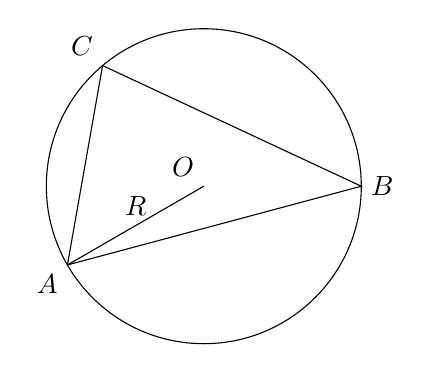
\begin{tikzpicture}
    \coordinate (O) at (0,0);
    \coordinate (B) at (0:2cm);
    \coordinate (A) at (210:2cm);
    \coordinate (C) at (130:2cm);
    
    \draw (O) circle (2cm);
    \draw (A) -- (B) -- (C) -- cycle;
    \node[right] at (B) {$B$};
    \node[below left] at (A) {$A$};
    \node[above left] at (C) {$C$};
    \node[above left] at (O) {$O$};
    \draw (A) -- node[above]{$R$} (O);
    \end{tikzpicture}
\end{center}
    \subsubsection{Dalil Sinus}
    $$\dfrac{BC}{\sin \angle A} = \dfrac{CA}{\sin \angle B}= \dfrac{AB}{\sin \angle C} = 2R$$
    
    \subsubsection{Dalil Cosinus}
    \begin{align*}
        AB^2 &= BC^2 + CA^2 - 2\cdot BC \cdot CA \cdot \cos \angle C\\
        BC^2 &= CA^2 + AB^2 - 2\cdot CA \cdot AB \cdot \cos \angle A\\
        CA^2 &= AB^2 + BC^2 - 2\cdot AB \cdot BC \cdot \cos \angle B
    \end{align*}
\subsection{Dalil Stewart}
    Pada segitiga $ABC$ dengan titik $D$ pada segmen $BC$, dimana $AB=c, BC=a, CA=b, AD=d, BD=m, CD=n$, maka berlaku
    $$BC \cdot AD^2 + BC \cdot BD \cdot CD = CA^2 \cdot BD + AB^2 \cdot CD$$
    atau $$ad^2+amn = b^2m+c^2n.$$

\subsection{Latihan Soal Dalil Stewart}
\begin{enumerate}
    \item (OSK 2016) Pada segitiga $ABC$, titik $M$ terletak pada $BC$ sehingga $AB=7, AM=3, BM=5$, dan $MC=6$. Panjang $AC$ adalah \dots
\end{enumerate}
\subsection{Dalil Ceva}
Jika pada segitiga $ABC$, titik $D,E,F$ berturut-turut berada di segmen $BC$,$CA$,$AB$, maka 
$AD,BE,CF$ konkuren atau berpotongan di satu titik jika dan hanya jika $$\dfrac{AF}{FB} \cdot \dfrac{BD}{DC} \cdot \dfrac{CE}{EA} = 1.$$
\begin{center}
    \begin{tikzpicture}
    % titik-titik segitiga
    \coordinate[label=left:$A$]  (A) at (-1.5cm,-1.cm);
    \coordinate[label=right:$B$] (B) at (1.5cm,-1.0cm);
    \coordinate[label=above:$C$] (C) at (0.5cm,1.732cm);
    
    % pembuatan segitiga
    \draw (A) -- (B) -- (C) -- cycle;
    
    % titik-titik cevian
    \coordinate[label=below:$F$] (F) at ($(A)!0.7!(B)$);
    \coordinate[label=right:$D$] (D) at ($(B)!0.5!(C)$);
    \coordinate[label=left:$E$]  (E) at ($(C)!0.3!(A)$);
    
    % pembuatan cevian
    \draw (A) -- (D);
    \draw (B) -- (E);
    \draw (C) -- (F);
    \end{tikzpicture}
\end{center}
\subsection{Dalil Menelaus}
Jika pada segitiga $ABC$, titik $P,Q,R$ berturut-turut berada pada garis (bisa di perpanjangan segmen) $BC$,$CA$, $AB$, maka $P,Q,R$ segaris jika dan hanya jika
$$\dfrac{AR}{RB} \cdot \dfrac{BP}{PC} \cdot \dfrac{CQ}{QA} = 1.$$
\begin{center}
    \begin{asy}
        unitsize(10);
        defaultpen(fontsize(8));
        pair P=(7,6), Q=(0,0), C=(10,0), A=(4,0), B=(6,8), R;
        draw((A)--(B)--(C)--cycle,blue+0.75);
        draw(P--R--Q--A);
        R=intersectionpoint(A--B,Q--P);
        dot(A^^B^^C^^P^^Q^^R);
        label("A",A,(0,-1));label("B",B,(1,0));label("C",C,(1,0));label("P",P,(1,1));label("Q",Q,(-1,0));label("R",R,(-1,1));
    \end{asy}
\end{center}
\subsection{Latihan Soal Dalil Menelaus}
\begin{enumerate}
    \item Dalam segitiga $ABD$, $F$ berada pada segmen $AD$, $E$ berada pada sinar $BF$, $G$ berada pada segmen $BD$, dan $C$ adalah titik perpotongan dari $FG$ dan $ED$. Diketahui bahwa $AB = 15$, $BD = 18$, $AF = 15$, $DF = 12$, $BE = 24$, dan $CF = 17$. Temukan rasio $BG : FG$.
    % https://drive.google.com/drive/search?q=parent:0B-4OltLGFEDFeG92VENBbmdZODA%20type:pdf%20menelaus

    \item (OSK 2022) Diberikan $ABC$ siku-siku sama kaki dengan $BC=AB$. Misalkan $L$ titik tengah $BC$ dan $P$ pada sisi $AC$ sehingga $BP \perp AL$. Jika $CP=30\sqrt{2}$, maka panjang $AB$ adalah \ldots

    \item Diberikan segitiga $ABC$ dengan panjang $BC = 36$. Misalkan $D$ adalah titik tengah $BC$ dan $E$ adalah titik tengah $AD$. Misalkan pula bahwa $F$ adalah perpotongan $BE$ dengan $AC$. Jika diketahui bahwa $AB$ menyinggung lingkaran luar segitiga $BFC$, hitunglah panjang $BF$.
\end{enumerate}
\subsection{Dalil Ptolemy}
    Diketahui sebuah segiempat siklis $ABCD$ maka berlaku
    $$AB \cdot CD + BC \cdot DA = AC \cdot BD.$$

\begin{center}
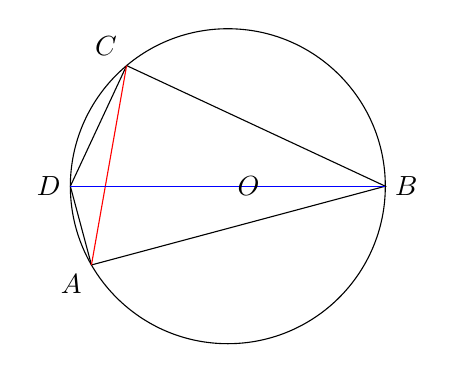
\begin{tikzpicture}
\coordinate (O) at (0,0);
\coordinate (B) at (0:2cm);
\coordinate (A) at (210:2cm);
\coordinate (D) at (180:2cm);
\coordinate (C) at (130:2cm);

\draw (O) circle (2cm);

\draw (A) -- (B) -- (C) -- (D) -- cycle;
\draw[red] (A) -- (C);
\draw[blue] (B) -- (D);

\node[right] at (B) {$B$};
\node[below left] at (A) {$A$};
\node[left] at (D) {$D$};
\node[above left] at (C) {$C$};
\node[right] at (O) {$O$};
\end{tikzpicture}
\end{center}

\subsection{Latihan Soal Dalil Ptolemy}
\begin{enumerate}
    \item Diberikan sebuah segiempat siklis $ABCD$ dengan $ABC$ adalah segitiga sama sisi. Jika $AD=2$ dan $CD=3$, panjang $BD=\dots$
\end{enumerate}
\subsection{Teorema Garis Bagi}
Misalkan garis bagi sudut $\angle A$ (bisa garis bagi dalam atau garis bagi luar) memotong garis $BC$ di $K$, maka 
$$\dfrac{BK}{CK} = \dfrac{AB}{AC}.$$
\begin{center}
    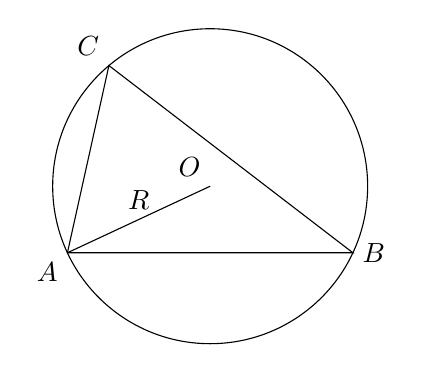
\begin{tikzpicture}
        \coordinate (O) at (0,0);
        \coordinate (B) at (-25:2cm);
        \coordinate (A) at (205:2cm);
        \coordinate (C) at (130:2cm);
        \coordinate (D) at (-90:2cm);
        
        \draw (O) circle (2cm);
        \draw (A) -- (B) -- (C) -- cycle;
        \node[right] at (B) {$B$};
        \node[below left] at (A) {$A$};
        \node[above left] at (C) {$C$};
        \node[above left] at (O) {$O$};
        \draw (A) -- node[above]{$R$} (O);
    \end{tikzpicture}
\end{center}
\subsection{Latihan Soal Teorema Garis Bagi}
\begin{enumerate}
    \item (OSK 2014) Diberikan segitiga $ABC$ dengan $AB = 360, BC = 240,$ dan $AC = 180$. Garis bagi dalam dan garis bagi luar dari $\angle CAB$ memotong $BC$ dan perpanjangan $BC$ berturut-turut di $P$ dan $Q$. Jari-jari lingkaran yang melalui titik-titik $A, P,$ dan $Q$ adalah \dots
\end{enumerate}

\section{Referensi}
    \begin{enumerate}
        \item Hermanto, Eddy. 2011. Diktat Pembinaan Olimpiade Matematika Dasar.
    \end{enumerate}



